\documentclass[12pt]{scrartcl}
\usepackage{amsmath, amssymb, amsthm, mathtools,amsthm}
\newtheorem{theorem}{Theorem}[section]
\newtheorem{corollary}{Corollary}[theorem]
\newtheorem{lemma}[theorem]{Lemma}

\usepackage{enumitem}
\usepackage{tikz, pgfplots}
\pgfplotsset{compat=1.17, width=10cm}
\usepgfplotslibrary{external}
\tikzexternalize

\usepackage{siunitx}

\usepackage[OT1]{fontenc}
\usepackage{mlmodern}
\usepackage{setspace}

\usepackage[backend=biber,style=numeric,sortcites=true]{biblatex}
\addbibresource{main.bib}
\usepackage{hyperref}

\title{The Bigger The Better II}
\author{Group 8-29 \thanks{Derrick Lukimin (L, 2i204), Tan Yong Yih (2i222), Wu Hao (2i324), Darren Yap (2i425)}}
\date{2022}

\begin{document}
\onehalfspacing
\maketitle
\tableofcontents

\section{Introduction}
This project aims to find an algorithm to determine
the side length of the largest square that can be
inscribed inside a convex $n$-gon. It is a continuation from
a previous project completed in 2021, The Bigger The Better. \cite{tbtb1}

\subsection{Definitions}
\begin{description}[font=\bfseries, leftmargin=1cm, style=nextline]
	\item[placement] A valid location, size and rotation of the square such that
		all vertices of the square lie on the edges of the polygon.
	\item[inscribed] All vertices of the square must lie on the edges of the polygon.
	\item[RQ] Research Question
\end{description}

\subsection{Research Questions}
\begin{enumerate}
	\item What is the side length of the largest square that can be inscribed in a triangle?
	\item What is the side length of the largest square that can be inscribed in a regular $n$-gon, given $n \neq 4$?
	\item What is the side length of the largest square that can be inscribed in a convex $n$-gon?
\end{enumerate}

\subsection{Project Scope}
This project will only focus on convex polygons.

\section{Literature Review}
% stuff...

\section{Research Question 1}

RQ1 aims to find out the side length of the largest square that can be inscribed in a triangle,
given the side lengths of the triangle, $a$, $b$ and $c$.

\subsection{Key Insights}
Some key insights which greatly aided in solving this problem were found.
\begin{enumerate}
	\item It can be seen that no more than two vertices of a square can lie on a single side,
	      as a square has at most two co-linear vertices.
	\item We notice how a triangle has three sides, and a square has four vertices.
	      In order for all the vertices to lie on the triangle, using the Pigeonhole Principle,
	      there will be at least one side with two vertices lying on it.
	\item Combining the above insights, there will be one vertex of the square
	      each lying on two sides of the triangle, with the other two vertices of the square
	      lying on the latter side of the triangle.
\end{enumerate}

\subsection{Solution}
A figure has been constructed for the purposes of illustrating the following proof.
\begin{figure}[htpb]
	\centering
	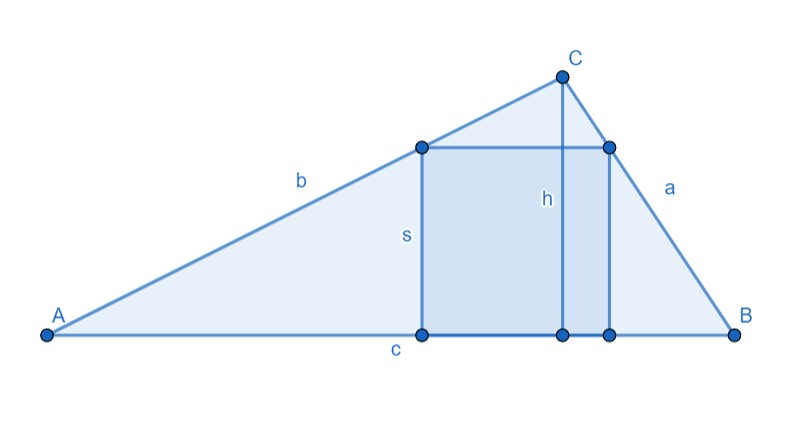
\includegraphics[scale=.75]{images/rq1.jpg}
	\label{fig:rq1_img}
	\caption{The figure for RQ1.}
\end{figure}
Let $s$ be the side length of the largest square that can be inscribed in a triangle,
with side lengths $a$, $b$ and $c$, and circumradius $R$.

Side $c$ can be formed with the sum of $s$, $s \cot A$ and $s \cot \angle{B}$. Hence, we can express $s$ with the side length $c$, as well as angles $A$ and $B$.
\begin{align*}
	c & = s+s\cot \angle{A}+s\cot \angle{B}          \\
	s & = \frac{c}{1+\cot \angle{A}+\cot \angle{B}}                                                                            
\end{align*}
We multiply both sides of the fraction by $\sin A \sin B$ and use the sine addition formula.
\begin{align*}
	s & = \frac{c \sin\angle{A}}{\sin\angle{A}+\cos\angle{A}+\cot\angle{B}\sin\angle{A}}                                       \\
	  & = \frac{c\sin\angle{A}\sin\angle{B}}{\sin\angle{A}\sin\angle{B}+\cos\angle{A}\sin\angle{B}+\sin\angle{A}\cos\angle{B}} \\
	  & = \frac{c\sin\angle{A}\sin\angle{B}}{\sin\angle{A}\sin\angle{B}+\sin\left(\angle{A}+\angle{B}\right)}                  \\
	  & = \frac{c\sin\angle{A}\sin\angle{B}}{\sin\angle{A}\sin\angle{B}+\sin\left(180-\angle C\right)}                         \\
	  & = \frac{c\sin\angle{A}\sin\angle{B}}{\sin\angle{A}\sin\angle{B}+\sin \angle C}                                         
\end{align*}
Now, we can multiply both sides of the fraction to $2Rc$ and use the law of sines to simplify.
	  & = \frac{2Rc\sin\angle{A}\sin\angle{B}}{2R\sin\angle{A}\sin \angle{B}+2R\sin \angle C}                                  \\
	  & = \frac{ac\sin\angle{B}}{a\sin\angle{B}+c}                                                                             \\
	  & = \frac{2Rac\sin\angle{B}}{2Ra\sin\angle{B}+2Rc}                                                                       \\
	  & = \frac{abc}{2Rc+ab}
\end{align*}
% We used formulae and theorems such as the sine addition formula and the law of sines to manipulate the expressions. \\

Since each of the sides of the triangle, $a$, $b$ and $c$ can be the longest side,
the maximum of the three placements can be taken as the solution, hence
\begin{equation}
	s_{\text{max}} = \max\left(\dfrac{abc}{2Rc+ab},\dfrac{abc}{2Rb+ac},\dfrac{abc}{2Ra+bc}\right)
\end{equation}

For obtuse triangles, only one placement exists, i.e. when the square lies on the longest side.
\begin{equation}
	s = \dfrac{abc}{2Rc+ab}
\end{equation}
where $c$ is the longest side.

\section{Research Question 2}

RQ2 aims to find out the side length of the largest square that can be inscribed in a convex $n$-gon,
given $n$ and the side length of the $n$-gon, $k$.

This problem can be further split into three cases.
\begin{enumerate}
	\item when $n$ is divisible by $4$,
	\item when $n$ is divisible by $2$ but not $4$,
	\item when $n$ is not divisible by $2$.
\end{enumerate}

\subsection{Case 1}
This case deals with the scenario where the number of sides in the $n$-gon is
divisible by $4$.

It can be seen that the diagonal of the square must be equal to the diagonal of the polygon.
\begin{proof}
	The diagonal of the square connects two vertices of the square opposite to each other.
	It is the longest line segment within a square.
	Since the square must be inscribed in the polygon, both ends of the diagonal have to lie on the edges of the polygon.
	The two furthest points on the edges of the polygon would be any vertex of the polygon and the vertex opposite to it.
	Hence, the diagonal of the square can be at most the length of the diagonal of the polygon.
\end{proof}

Such a construction exists, as shown by the following figure.
\begin{figure}[htpb]
	\centering
	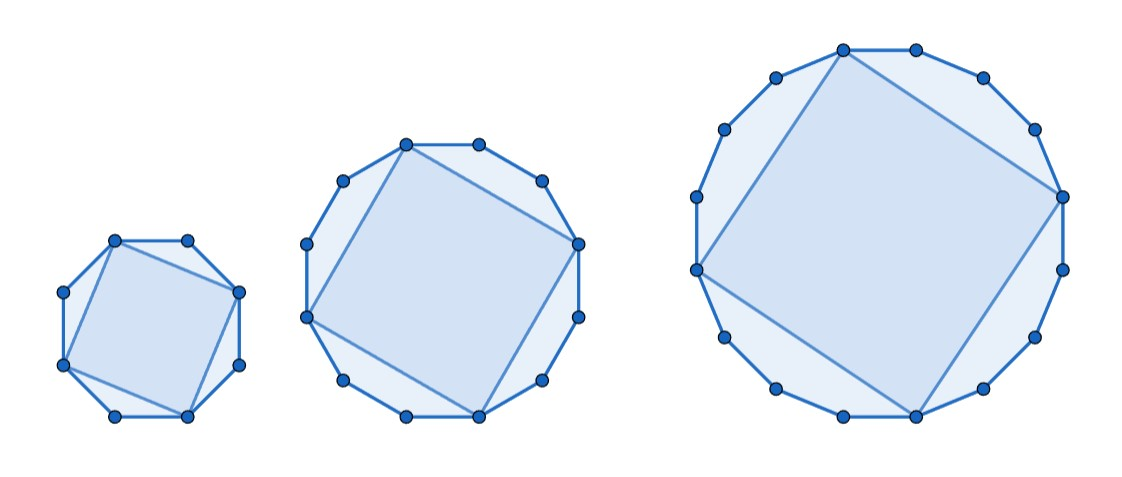
\includegraphics[scale=.65]{images/rq2_1_1.jpg}
	\label{fig:rq2_1_1_img}
	\caption{The constructions for Case 1 of RQ2.}
\end{figure}

Hence, the side length of the square can be calculated.
With reference to the figure, the Law of Cosines can be applied.

\begin{theorem}[Law of Cosines]
	Given a triangle with side lengths $a$, $b$ and $c$, and the angle formed by $a$
	and $b$ as $\gamma$, $a^2 + b^2 - 2ab \cos \gamma = c^2$.
\end{theorem}

\begin{figure}[htpb]
	\centering
	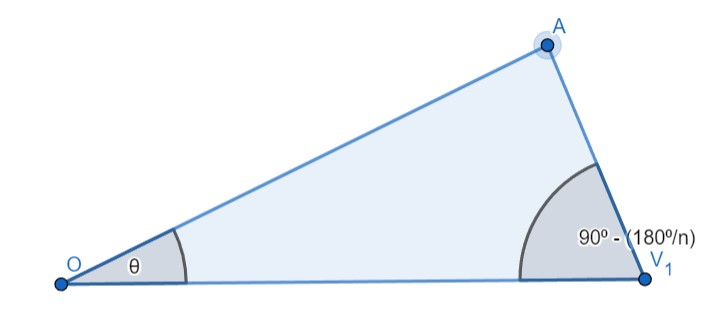
\includegraphics[scale=.75]{images/rq2_1_2.jpg}
	\label{fig:rq2_1_2_img}
	\caption{The figure for case 1 of RQ2.}
\end{figure}

Taking $n$ to be the number of sides in the $n$-gon, $k$ to be the side length
of the $n$-gon, and $l$ to be the distance from a vertex of the $n$-gon to its midpoint:
\begin{align*}
	\angle{AMB}                                               & = \frac{\ang{360}}{n}                                          \\
	l^2+l^2-2\left(l\right)\left(l\right)\cdot\cos\angle{AMB} & =k^{2}                                                         \\
	2l^2\left(1-\cos\angle{AMB}\right)                        & =k^{2}                                                         \\
	l^2                                                       & =\frac{k^{2}}{2\left(1-\cos{\frac{\ang{360}}{n}}\right)}       \\
	l                                                         & =\ k\sqrt{\frac{1}{2\left(1-\cos{\frac{\ang{360}}{n}}\right)}} \\
\end{align*}

Using the Pythagorean Theorem, which stipulates that:
\begin{theorem}[Pythagorean Theorem]
	In a right-angled triangle with side lengths $a$, $b$ and $c$, $c$ being that of the hypotenuse,
	$a^2 + b^2 = c^2$.
\end{theorem}

\begin{align*}
	2s^{2} & = \left(2l\right)^{2}                                         \\
	s^{2}  & = 2l^{2}                                                      \\
	s      & = l\sqrt{2}                                                   \\
	       & = k\sqrt{\frac{2}{2\left(1-\cos{\frac{\ang{360}}{n}}\right)}} \\
	       & = k\sqrt{\frac{1}{\left(1-\cos{\frac{\ang{360}}{n}}\right)}}  \\
\end{align*}

Hence,
\begin{equation}
	s = k\sqrt{\frac{1}{\left(1-\cos{\frac{\ang{360}}{n}}\right)}}
\end{equation}

\printbibliography
\end{document}
